\documentclass[tikz,border=15pt]{standalone}
\usepackage{amsmath}
\usepackage{amssymb}
\usetikzlibrary{shapes.geometric,arrows.meta,positioning,calc}

% Define premium colors
\definecolor{predcolor}{HTML}{1A5B8C}   % Time Update / Prediction (Deep Blue)
\definecolor{upcolor}{HTML}{8C1A5B}     % Measurement Update (Berry)
\definecolor{meascolor}{HTML}{D97706}   % Measurement (Amber)
\definecolor{gaincolor}{HTML}{DC2626}   % Kalman Gain (Red)
\definecolor{statecolor}{HTML}{16A34A}  % State Estimate (Green)

% Soft zone colors for background separation
\definecolor{zonepred}{HTML}{EFF6FF}    % Soft blue
\definecolor{zoneupdate}{HTML}{FDF2F8}  % Soft pink/berry
\definecolor{zonemeas}{HTML}{FEF3C7}    % Soft amber
\definecolor{zoneest}{HTML}{F0FDF4}     % Soft green

\begin{document}
\renewcommand{\familydefault}{\sfdefault}
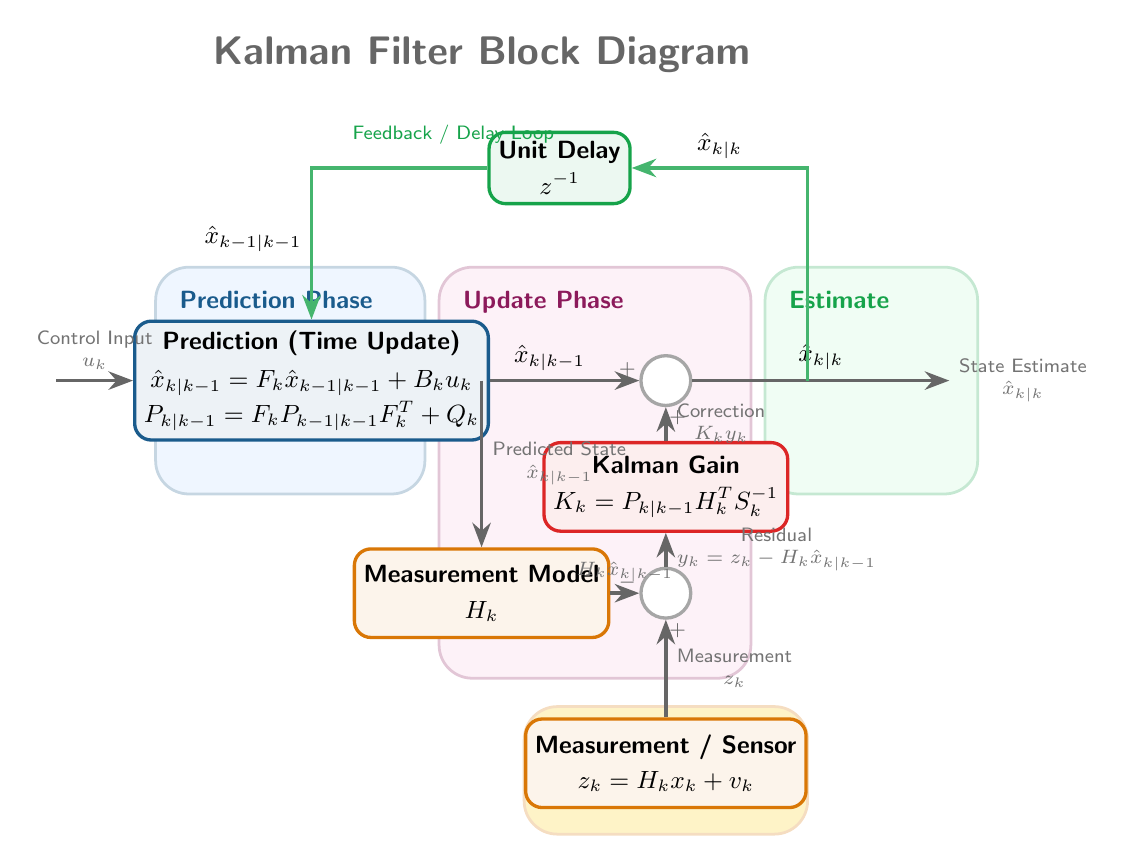
\begin{tikzpicture}[
    x=1.8cm, y=1.8cm,
    >=Stealth,
    block/.style={
        rectangle, 
        draw, 
        minimum height=3.2em, 
        minimum width=7.5em, 
        rounded corners=6pt, 
        align=center, 
        line width=1.2pt,
        font=\sffamily\small
    },
    predblock/.style={block, draw=predcolor, fill=predcolor!8},
    upblock/.style={block, draw=upcolor, fill=upcolor!8},
    gainblock/.style={block, draw=gaincolor, fill=gaincolor!8, minimum width=6em},
    measblock/.style={block, draw=meascolor, fill=meascolor!8},
    delayblock/.style={block, draw=statecolor, fill=statecolor!8, minimum width=5em, minimum height=2.5em},
    sum/.style={
        circle, 
        draw=gray!70, 
        fill=white, 
        minimum size=1.8em, 
        inner sep=0pt, 
        line width=1.2pt
    },
    flowline/.style={draw=gray!80!black, ->, line width=1.3pt},
    feedbackline/.style={draw=statecolor!80, ->, line width=1.3pt},
    labelstyle/.style={font=\sffamily\scriptsize\color{gray!90!black}, align=center},
    mathlabel/.style={font=\sffamily\small\color{black}}
]

% Place layers for clean background drawing
\pgfdeclarelayer{background}
\pgfdeclarelayer{foreground}
\pgfsetlayers{background,main,foreground}

% --- COORDINATES & NODES ---

% Inputs
\coordinate (control_in) at (-1.8, 0);

% Prediction Block
\node[predblock] (pred) at (0, 0) {
    \textbf{Prediction (Time Update)}\\[0.3em]
    $\hat{x}_{k|k-1} = F_k \hat{x}_{k-1|k-1} + B_k u_k$\\[0.2em]
    $P_{k|k-1} = F_k P_{k-1|k-1} F_k^T + Q_k$
};

\coordinate (branch_pred) at (1.2, 0);

% Update Phase Elements
\node[sum] (sum_state) at (2.5, 0) {};

\coordinate (branch_est) at (3.5, 0);
\coordinate (state_out) at (4.5, 0);

% Measurement & Model Elements
\node[measblock] (meas_matrix) at (1.2, -1.5) {
    \textbf{Measurement Model}\\[0.2em]
    $H_k$
};

\node[sum] (sum_meas) at (2.5, -1.5) {};

\node[measblock] (sensor) at (2.5, -2.7) {
    \textbf{Measurement / Sensor}\\[0.2em]
    $z_k = H_k x_k + v_k$
};

% Kalman Gain Block
\node[gainblock] (gain) at (2.5, -0.75) {
    \textbf{Kalman Gain}\\[0.2em]
    $K_k = P_{k|k-1} H_k^T S_k^{-1}$
};

% Feedback Delay Block
\node[delayblock] (delay) at (1.75, 1.5) {
    \textbf{Unit Delay}\\[0.2em]
    $z^{-1}$
};

% --- BACKGROUND ZONES ---
\begin{pgfonlayer}{background}
    % Prediction Zone
    \fill[zonepred, draw=predcolor!25, line width=1pt, rounded corners=12pt] 
        (-1.1, -0.8) rectangle (0.8, 0.8);
    \node[anchor=north west, predcolor, font=\sffamily\bfseries\small] at (-1.0, 0.7) {Prediction Phase};

    % Update Zone
    \fill[zoneupdate, draw=upcolor!25, line width=1pt, rounded corners=12pt] 
        (0.9, -2.1) rectangle (3.1, 0.8);
    \node[anchor=north west, upcolor, font=\sffamily\bfseries\small] at (1.0, 0.7) {Update Phase};

    % Measurement Zone
    \fill[zonemeas, draw=meascolor!25, line width=1pt, rounded corners=12pt] 
        (1.5, -3.2) rectangle (3.5, -2.3);
    \node[anchor=north west, meascolor, font=\sffamily\bfseries\small] at (1.6, -2.4) {Measurement};

    % State Estimate Zone
    \fill[zoneest, draw=statecolor!25, line width=1pt, rounded corners=12pt] 
        (3.2, -0.8) rectangle (4.7, 0.8);
    \node[anchor=north west, statecolor, font=\sffamily\bfseries\small] at (3.3, 0.7) {Estimate};
\end{pgfonlayer}

% --- PATHS & ARROWS ---

% Control input to Prediction
\draw[flowline] (control_in) -- (pred.west)
    node[midway, above, labelstyle] {Control Input\\$u_k$};

% Prediction to Sum State & Branch to Measurement Model
\draw[flowline] (pred.east) -- (sum_state.west);
\draw[flowline] (branch_pred) -- (meas_matrix.north)
    node[midway, right, labelstyle] {Predicted State\\$\hat{x}_{k|k-1}$};

% Label on the horizontal line between pred and sum_state
\node[above, mathlabel] at ($(pred.east)!0.4!(sum_state.west)$) {$\hat{x}_{k|k-1}$};

% Measurement model to Measurement Sum
\draw[flowline] (meas_matrix.east) -- (sum_meas.west)
    node[midway, above, labelstyle] {$H_k \hat{x}_{k|k-1}$};

% Sensor to Measurement Sum
\draw[flowline] (sensor.north) -- (sum_meas.south)
    node[midway, right, labelstyle] {Measurement\\$z_k$};

% Measurement Sum to Kalman Gain
\draw[flowline] (sum_meas.north) -- (gain.south)
    node[midway, right, labelstyle] {Residual\\$y_k = z_k - H_k \hat{x}_{k|k-1}$};

% Kalman Gain to State Sum
\draw[flowline] (gain.north) -- (sum_state.south)
    node[midway, right, labelstyle] {Correction\\$K_k y_k$};

% Sum State to Output
\draw[flowline] (sum_state.east) -- (state_out)
    node[midway, above, mathlabel] {$\hat{x}_{k|k}$};
\node[anchor=west, labelstyle] at (state_out) {State Estimate\\$\hat{x}_{k|k}$};

% Feedback loop
\draw[feedbackline] (branch_est) -- (branch_est |- delay.east) -- (delay.east);
\draw[feedbackline] (delay.west) -- (0, 1.5) -- (pred.north);

% Feedback labels
\node[above, mathlabel] at ($(branch_est |- delay.east)!0.5!(delay.east)$) {$\hat{x}_{k|k}$};
\node[left, mathlabel] at (0, 1.0) {$\hat{x}_{k-1|k-1}$};
\node[above, labelstyle, statecolor] at (1.0, 1.6) {Feedback / Delay Loop};

% Signs on Sums
\node[above left, inner sep=1pt, font=\sffamily\scriptsize\color{gray!80!black}] at (sum_state.west) {$+$};
\node[below right, inner sep=1pt, font=\sffamily\scriptsize\color{gray!80!black}] at (sum_state.south) {$+$};

\node[above left, inner sep=1pt, font=\sffamily\scriptsize\color{gray!80!black}] at (sum_meas.west) {$-$};
\node[below right, inner sep=1pt, font=\sffamily\scriptsize\color{gray!80!black}] at (sum_meas.south) {$+$};

% Title or Diagram Header
\node[align=center, font=\sffamily\Large\bfseries\color{gray!80!black}] at (1.2, 2.3) {Kalman Filter Block Diagram};

\end{tikzpicture}
\end{document}
